\documentclass{article}
\usepackage{amsmath}
\usepackage[a4paper, left=1in, right=1in, top=1in, bottom=1in]{geometry}
\everymath{\displaystyle}
\usepackage{tikz}
\usetikzlibrary{positioning,calc} % Для удобного позиционирования узлов

\begin{document}

\section*{Definition}

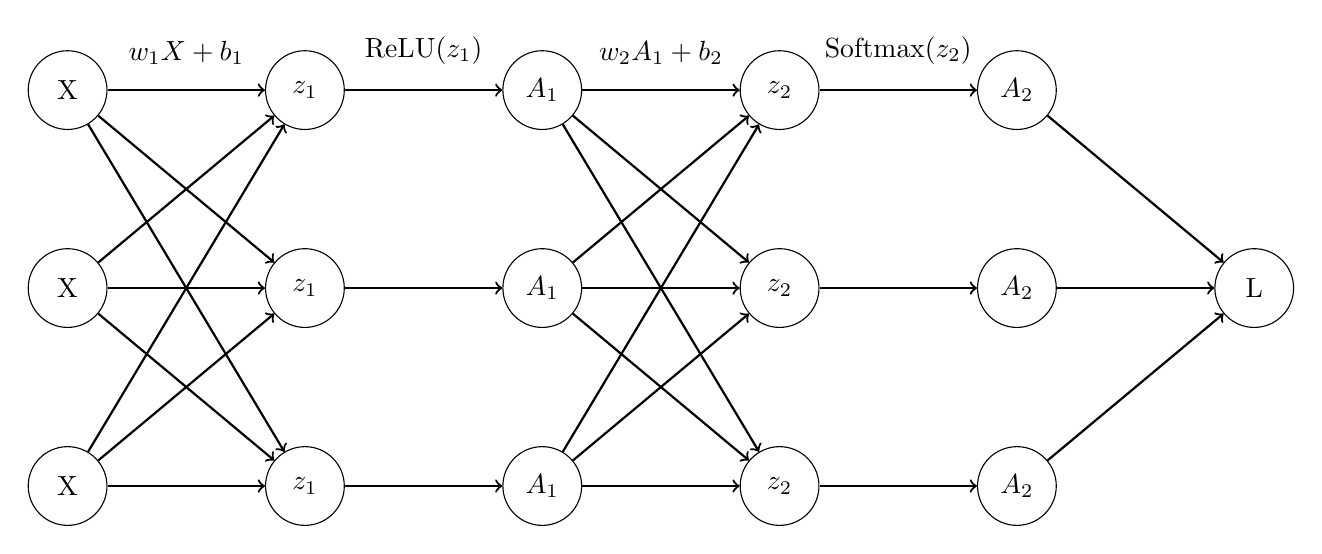
\begin{tikzpicture}[
    node distance=1.5cm and 2cm, % Расстояние между нейронами и слоями
    neuron/.style={circle, draw, minimum size=1cm}, % Стиль нейронов
    arrow/.style={->, thick} % Стиль стрелок
    ]

    % Входной слой
    \node[neuron] (X1) {X};
    \node[neuron, below=of X1] (X2) {X};
    \node[neuron, below=of X2] (X3) {X};

    % Полносвязный слой Z1
    \node[neuron, right=of X1] (Z1_1) {$z_1$};
    \node[neuron, below=of Z1_1] (Z1_2) {$z_1$};
    \node[neuron, below=of Z1_2] (Z1_3) {$z_1$};

    % Слой активации A1
    \node[neuron, right=of Z1_1] (A1_1) {$A_1$};
    \node[neuron, below=of A1_1] (A1_2) {$A_1$};
    \node[neuron, below=of A1_2] (A1_3) {$A_1$};

    % Полносвязный слой Z2
    \node[neuron, right=of A1_1] (Z2_1) {$z_2$};
    \node[neuron, below=of Z2_1] (Z2_2) {$z_2$};
    \node[neuron, below=of Z2_2] (Z2_3) {$z_2$};

    % Слой активации A2
    \node[neuron, right=of Z2_1] (A2_1) {$A_2$};
    \node[neuron, below=of A2_1] (A2_2) {$A_2$};
    \node[neuron, below=of A2_2] (A2_3) {$A_2$};

    % Функция потерь L
    \node[neuron, right=of A2_2] (L) {L};

    % Связи между слоями (входной -> Z1)
    \foreach \i in {1,2,3}
        \foreach \j in {1,2,3}
            \draw[arrow] (X\i) -- (Z1_\j);

    % Связи между слоями Z1 -> A1
    \foreach \i in {1,2,3}
        \draw[arrow] (Z1_\i) -- (A1_\i);

    % Связи между слоями A1 -> Z2
    \foreach \i in {1,2,3}
        \foreach \j in {1,2,3}
            \draw[arrow] (A1_\i) -- (Z2_\j);

    % Связи между слоями Z2 -> A2
    \foreach \i in {1,2,3}
        \draw[arrow] (Z2_\i) -- (A2_\i);

    % Связи между A2 и функцией потерь L
    \foreach \i in {1,2,3}
        \draw[arrow] (A2_\i) -- (L);

    % Подписи ребер (веса и смещения)
    \node[above=0.2cm of $(X1)!0.5!(Z1_1)$] {$w_1 X + b_1$};
    \node[above=0.2cm of $(Z1_1)!0.5!(A1_1)$] {$\text{ReLU}(z_1)$};
    \node[above=0.2cm of $(A1_1)!0.5!(Z2_1)$] {$w_2 A_1 + b_2$};
    \node[above=0.2cm of $(Z2_1)!0.5!(A2_1)$] {$\text{Softmax}(z_2)$};

\end{tikzpicture}

\begin{align*}
z_1 &= w_1 X + b_1 \\
A_1 &= \text{ReLU}(z_1) = \begin{cases}
z_{1i}, z_{1i} \geq 0 \\
0, z_{1i} < 0
\end{cases}\\
z_2 &= w_2 A_1 + b_2 \\
A_2 &= \text{Softmax}(z_2) = \frac{e^{z_{2i}}}{\sum_{j=1}^K e^{z_{2j}}} \\
L &= -\sum_{i=0}^{K} y_{ti} \log A_{2i} \\
\end{align*}

\section*{Gradients}

\begin{align*}
\frac{\partial L}{\partial w_2} ,
\frac{\partial L}{\partial b_2} ,
\frac{\partial L}{\partial w_1} ,
\frac{\partial L}{\partial b_1} - ?
\end{align*}

\begin{align*}
\frac{\partial L}{\partial w_{2i}} &= \frac{\partial L}{\partial A_{2i}} \cdot \frac{\partial A_{2i}}{\partial w_{2i}} = \frac{\partial L}{\partial A_{2i}} \cdot \frac{\partial A_{2i}}{\partial z_{2i}} \cdot \frac{\partial z_{2i}}{\partial w_{2i}} \\
\frac{\partial z_{2i}}{\partial w_{2i}} &= \frac{\partial}{\partial w_{2i}} (w_{2i} A_{1i} + b_2) = A_{1i}
\end{align*}

\begin{align*}
\frac{\partial L}{\partial z_{2i}} = \frac{\partial L}{\partial A_{2i}} \frac{\partial A_{2i}}{\partial z_{2i}} = \frac{\partial}{\partial A_{2i}} \left( -\sum_{i=0}^{K} y_{ti} \log A_{2i} \right) \frac{\partial A_{2i}}{\partial z_{2i}} = -\frac{y_{ti}}{A_{2i}} \frac{\partial}{\partial z_{2i}}  \left( \frac{e^{z_{2i}}}{\sum_{j=0}^{K} e^{z_{2j}}} \right) \overset{(1)}{=} \\
= \begin{cases}
-\frac{y_{ti}}{A_{2i}} \frac{A_{2i} \cdot \sum_{j=0}^{K} e_{z_{2j}} - e_{z_{2i}}}{\sum_{j=0}^{K} e_{z_{2j}}} , i = k \\
-\frac{y_{ti}}{A_{2i}} \frac{-A_{2i} \cdot e_{z_{2k}}}{\sum_{j=0}^{K} e_{z_{2j}}} , i \neq k
\end{cases} = \begin{cases}
-y_{ti} (1 - A_{2i}) , i = k \\
y_{ti} A_{2k} , i \neq k
\end{cases} \overset{(2)}{=} \\
= \begin{cases}
-I(y_{ti} = k) (1 - A_{2i}) , i = k \\
-I(y_{ti} = k) (0 - A_{2k}), i \neq k
\end{cases} = \begin{cases}
A_{2i} \cdot I(y_{ti} = k) - I(y_{ti} = k) , i = k \\
A_{2k} \cdot I(y_{ti} = k), i \neq k
\end{cases} \Leftrightarrow \\
\Leftrightarrow A_{2i} I(y_{ti} = k) - I(y_{ti} = k) + A_{2k} I(y_{ti} = k) =  A_{2i} - I(y_{ti} = k) = A_{2i} - y_{ti}
\end{align*}

\begin{align*}
(1) && \frac{\partial}{\partial z_{2i}}  \left( \frac{e^{z_{2i}}}{\sum_{j=0}^{K} e^{z_{2j}}} \right) &= \begin{cases}
\frac{\partial}{\partial z_{2i}}  \left( \frac{e^{z_{2i}}}{\sum_{j=0}^{K} e^{z_{2j}}} \right) , i = k \\
\frac{\partial}{\partial z_{2i}}  \left( \frac{e^{z_{2k}}}{\sum_{j=0}^{K} e^{z_{2j}}} \right) , i \neq k
\end{cases} = \begin{cases}
\frac{e^{z_{2i}} \left( \sum_{j=0}^{K} e^{z_{2j}} - e^{z_{2_i}} \right) }{\left( \sum_{j=0}^{K} e^{z_{2j}} \right)^2} , i = k \\
-\frac{e^{z_{2k}}}{\left( \sum_{j=0}^{K} e^{z_{2j}} \right)^2} \frac{\partial \left( \sum_{j=0}^{K} e^{z_{2j}} \right)}{\partial z_{2i}} , i \neq k
\end{cases} \\
&& \frac{\partial \left( \sum_{j=0}^{K} e^{z_{2j}} \right)}{\partial z_{2i}} &= e^{z_{2k}}, \frac{e^{z_{2i}}}{\left( \sum_{j=0}^{K} e^{z_{2j}} \right)^2} = A_{2i} \\
(2) && I(y_{ti} = k) &= y_{ti} 
\end{align*}

\begin{align*}
\boldsymbol{\frac{\partial L}{\partial w_{2i}}} &= (A_{2i} - y_{ti}) \cdot A_{1i} \\
\frac{\partial z_{2i}}{\partial b_2} &= 1 \\
\boldsymbol{\frac{\partial L}{\partial b_2}} &= \frac{\partial L}{\partial z_{2i}} \frac{\partial z_{2i}}{\partial b_2} = \frac{\partial L}{\partial z_{2i}} = A_{2i} - y_{ti}\\
\frac{\partial L}{\partial w_1} &= \frac{\partial L}{\partial z_{2i}}\frac{\partial z_{2i}}{\partial w_{1i}} = \frac{\partial L}{\partial z_{2i}} \frac{\partial z_{2i}}{\partial A_{1i}} \frac{\partial A_{1i}}{\partial z_{1i}} \frac{\partial z_{1i}}{\partial w_{1i}} \\
\frac{\partial z_{1i}}{\partial w_{1i}} &= X \\
\frac{\partial L}{\partial A_{1i}} &= \frac{\partial L}{\partial z_{2i}} w_1 = (A_{2i} - y_{ti}) \cdot w_1 \\
\frac{\partial A_{1i}}{\partial z_{1i}} &= \begin{cases}
1, z_{1i} \geq 0 \\
0, z_{1i} < 0
\end{cases} \\
\frac{\partial L}{\partial z_{1i}} &= \frac{\partial L}{\partial A_{1i}} \frac{\partial A_{1i}}{\partial z_{1i}} = \begin{cases}
(A_{2i} - y_{ti}) \cdot w_1 , z_{1i} \geq 0 \\
0, z_{1i} < 0
\end{cases} = (A_{2i} - y_{ti}) \cdot w_1 , z_{1i} \geq 0 \\
\frac{\partial z_{2i}}{\partial A_{1i}} &= w_2 \\
\boldsymbol{\frac{\partial L}{\partial w_{1i}}} &= (A_{2i} - y_{ti}) \cdot w_2 X \\
\frac{\partial z_{1i}}{\partial b_1} &= 1 \\
\boldsymbol{\frac{\partial L}{\partial b_1}} &= \frac{\partial L}{\partial z_{2i}} \frac{\partial z_{2i}}{\partial b_1} =  \frac{\partial L}{\partial z_{2i}} \frac{\partial z_{2i}}{\partial A_{1i}}  \frac{\partial A_{1i}}{\partial b_1} = \frac{\partial L}{\partial z_{2i}} \frac{\partial z_{2i}}{\partial A_{1i}} \frac{\partial A_{1i}}{\partial z_{1i}} \frac{\partial z_{1i}}{\partial b_1} = \frac{\partial L}{\partial z_{1i}} \frac{\partial z_{1i}}{\partial b_1} = \frac{\partial L}{\partial z_{1i}} \overset{z_{1i} \geq 0}{=} (A_{2i} - y_{ti}) \cdot w_1
\end{align*}

\end{document}
